\documentclass{beamer}
%
% Choose how your presentation looks.
% For more themes, color themes and font themes, see:
% http://deic.uab.es/~iblanes/beamer_gallery/index_by_theme.html
%
\mode<presentation>
{
  \usetheme{Madrid}      % or try Darmstadt, Madrid, Warsaw, ...
  \usecolortheme{seahorse} % or try albatross, beaver, crane, ...
  \usefonttheme{serif}  % or try serif, structurebold, ...
  \setbeamertemplate{navigation symbols}{}
  \setbeamertemplate{caption}[numbered]
  \usepackage{amsmath}
  \usepackage{tcolorbox}
  \usepackage[export]{adjustbox}
  \tcbuselibrary{most}
  \usepackage{arydshln}
  \usepackage{tikz}
  \usetikzlibrary{plotmarks}
  \usepackage{pgfplots}
  \newcommand{\Ivec}[1]{\mbox{\boldmath $#1$}}
    \usepackage[normalem]{ulem}
    % \usepackage{tipa}
    \newcommand{\git}{\texttt{\textbf{git}}\xspace}
    \usepackage{listings}
} 


\definecolor{myblue}{RGB}{65,105,225} 
\definecolor{myorange}{RGB}{250,190,0}

\setbeamercolor{structure}{fg=white,bg=myorange}
\setbeamercolor*{palette primary}{fg=myblue,bg=myorange}
\setbeamercolor*{palette secondary}{fg=white,bg=myblue}
\setbeamercolor*{palette tertiary}{bg=myblue,fg=white}
\setbeamercolor*{palette quaternary}{fg=white,bg=myorange!50}

\setbeamercolor{frametitle}{fg=black!90!myblue}

\setbeamercolor{section in head/foot}{fg=white,bg=myblue}
\setbeamercolor{author in head/foot}{fg=black,bg=myorange}
\setbeamercolor{title in head/foot}{fg=white,bg=myblue}

\setbeamertemplate{navigation symbols}{}

\setbeamertemplate{itemize/enumerate body begin}{\large}
\setbeamertemplate{itemize/enumerate subbody begin}{\large}


\defbeamertemplate*{headline}{mytheme}
{%
  \begin{beamercolorbox}[ht=2.25ex,dp=3.75ex]{section in head/foot}
    \insertnavigation{\paperwidth}
  \end{beamercolorbox}%
}%

\defbeamertemplate*{footline}{mytheme}
{
  \leavevmode%
  \hbox{%
  \begin{beamercolorbox}[wd=.5\paperwidth,ht=2.25ex,dp=1ex,right]{author in head/foot}%
    \usebeamerfont{author in head/foot}\insertshortauthor\hspace*{2em}
  \end{beamercolorbox}%
  \begin{beamercolorbox}[wd=.5\paperwidth,ht=2.25ex,dp=1ex,left]{title in head/foot}%
    \usebeamerfont{title in head/foot}\hspace*{2em}\insertshortsubtitle\hspace*{2em}
    \insertframenumber{} / \inserttotalframenumber
  \end{beamercolorbox}}%
  \vskip0pt%
}

\usepackage[english]{babel}
\usepackage[utf8x]{inputenc}
\usepackage{xcolor}
\usepackage{listings}
\usepackage{pgf}  
\usepackage{textpos}
\usepackage{tabulary}
\usepackage{scrextend}
\usepackage{hyperref}
\usepackage{setspace}
\usepackage{rotating}
\lstset
{
    language=[LaTeX]TeX,
    breaklines=true,
    basicstyle=\tt\scriptsize,
    %commentstyle=\color{green}
    keywordstyle=\color{blue},
    %stringstyle=\color{black}
    identifierstyle=\color{magenta},
}
\newcommand{\bftt}[1]{\textbf{\texttt{#1}}}
%\newcommand{\comment}[1]{{\color[HTML]{008080}\textit{\textbf{\texttt{#1}}}}}
\newcommand{\cmd}[1]{{\color[HTML]{008000}\bftt{#1}}}
\newcommand{\bs}{\char`\\}
\newcommand{\cmdbs}[1]{\cmd{\bs#1}}
\newcommand{\lcb}{\char '173}
\newcommand{\rcb}{\char '175}
\newcommand{\cmdbegin}[1]{\cmdbs{begin\lcb}\bftt{#1}\cmd{\rcb}}
\newcommand{\cmdend}[1]{\cmdbs{end\lcb}\bftt{#1}\cmd{\rcb}}

\newcommand{\wllogo}{\textbf{Overleaf}}

\usepackage{hyperref}
\hypersetup{
    colorlinks=true,
    linkcolor=blue,
    filecolor=magenta,      
    urlcolor=cyan,
    pdftitle={Overleaf Example},
    pdfpagemode=FullScreen,
    }

\urlstyle{same}

% this is where the example source files are loaded from
% do not include a trailing slash
\newcommand{\fileuri}{https://raw.githubusercontent.com/GiancarloSucci/UniBo.IDSEPC.A2022/main/A2022.IDSEPCLaTeX/}

\newcommand{\perche}{perch\'{e}}
\newcommand{\affinche}{affinch\'{e}}
\newcommand{\se}{s\'{e}}
\newcommand{\a}{\`{a}}
\newcommand{\est}{\`{e}}

\usepackage{stackengine}
\def\Ruble{\stackengine{.67ex}{%
  \stackengine{.48ex}{\textsf{P}}{\rule{.8ex}{.12ex}\kern.6ex}{O}{r}{F}{F}{L}%
  }{\rule{.8ex}{.12ex}\kern.6ex}{O}{r}{F}{F}{L}\kern-.1ex}



%----------------------------------------------------------------------------------------
%	TITLE PAGE
%----------------------------------------------------------------------------------------
\title[L02]{Introduzione alla data science e al pensiero computazionale\\
Lezione 7: Le Scale dei Dati} % The short title appears at the bottom of every slide, the full title is only on the title page

\author[{\tiny Giancarlo Succi }]{Giancarlo Succi\\\\ Dipartimento di Informatica -- Scienza e Ingegneria\\Universit\`{a} di Bologna\\
\bftt{g.succi@unibo.it}
} % Your name
\institute[unibo] % Your institution as it will appear on the bottom of every slide, may be shorthand to save space

\date{} % Date, can be changed to a custom date

\setbeamertemplate{navigation symbols}{}
\AtBeginSection[]
{
        \begin{frame}<beamer>{Outline}
                \tableofcontents[currentsection]
        \end{frame}
}

\begin{document}
\begin{frame}
\titlepage % Print the title page as the first slide

\end{frame}

%=============================================

\addtobeamertemplate{frametitle}{}{%
\begin{textblock*}{10mm}(-0.01mm,-0.95cm)

\includegraphics[width=0.9cm]{unibo-logo.png}
\end{textblock*}}

%=============================================


%=============================================
%---------------------------------------------
\begin{frame}{\centerline{Mapping}}

\begin{itemize}
\item Attribute values \(->\) numbers or symbols
\item Attribute value domain \(->\) range
\item Empirical relation \(->\) mathematical relation\\
\end{itemize}
\begin{center}
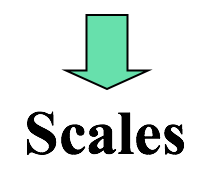
\includegraphics[width=20mm]{A2022.ScaleDeiDati/img-img14.png}
\end{center}

\end{frame}
%=============================================

%---------------------------------------------
\begin{frame}{\centerline{Measurement Scales}}

\begin{itemize}
\item A measurement scale is a class of mapping that links empirical and number relations with specific properties
\end{itemize}

\end{frame}
%=============================================

%---------------------------------------------
\begin{frame}{\centerline{Measurement Scales}}

\begin{itemize}
\item Best possible numerical relation system?
\item Representation of an empirical relation in a numerical system?
\item Choosing a unique (and best) number system?

\end{itemize}

\end{frame}
%=============================================

%---------------------------------------------
\begin{frame}{\centerline{Measurement Scales}}

\begin{itemize}

\item Qualitative Scales
\begin{itemize}
\item Nominal (gender)
\item Ordinal (arrival order)
\end{itemize}
\item Numeric/Continuous Scales
\begin{itemize}
\item Interval (temperatures in F)
\item Ratio (height)
\item Absolute (the actual count)
\end{itemize}
\end{itemize}

\end{frame}
%=============================================

%---------------------------------------------
\begin{frame}{\centerline{Measurement Scales}}

\begin{itemize}
\item Language(Program) = 1, if Program is written in Pascal
\item Language(Program) = 2, if Program is written in C
\item Language(Program) = 3, if Program is written in Fortran
\end{itemize}
\textit{Few mathematical operations are applicable (mode, histograms, …)}
\end{frame}
%=============================================

%---------------------------------------------
\begin{frame}{\centerline{Measurement Scales}}

\begin{itemize}
\item Difficult(Program) = 1, if Program is easy to read
\item Difficult(Program) = 2, if Program is not hard to read 
\item Difficult(Program) = 3, if Program is hard to read 
\end{itemize}
\textit{We can have the median here...}

\end{frame}
%=============================================

%---------------------------------------------
\begin{frame}{\centerline{Measurement Scales}}

\begin{itemize}
\item \underline{Nominal} measure label variables without any quantitative value. Ex., Eye color.
\item \underline{Ordinal} measure categorize data in natural order. Size of steps between items is unknown. Ex.,  Customer satisfaction 
\item \underline{Interval} measures preserve differences but not ratios. Ex., The absolute time when an event occurred.
\item \underline{Ratio} measures preserve also the ratio between entities. Ex., LOC in a program. \textit{All math operations are applicable.}
\item \underline{Absolute} measures are counts. Ex., the number of if statements in a program.
\end{itemize}

\end{frame}
%=============================================

%---------------------------------------------
\begin{frame}{\centerline{}}

\begin{center}
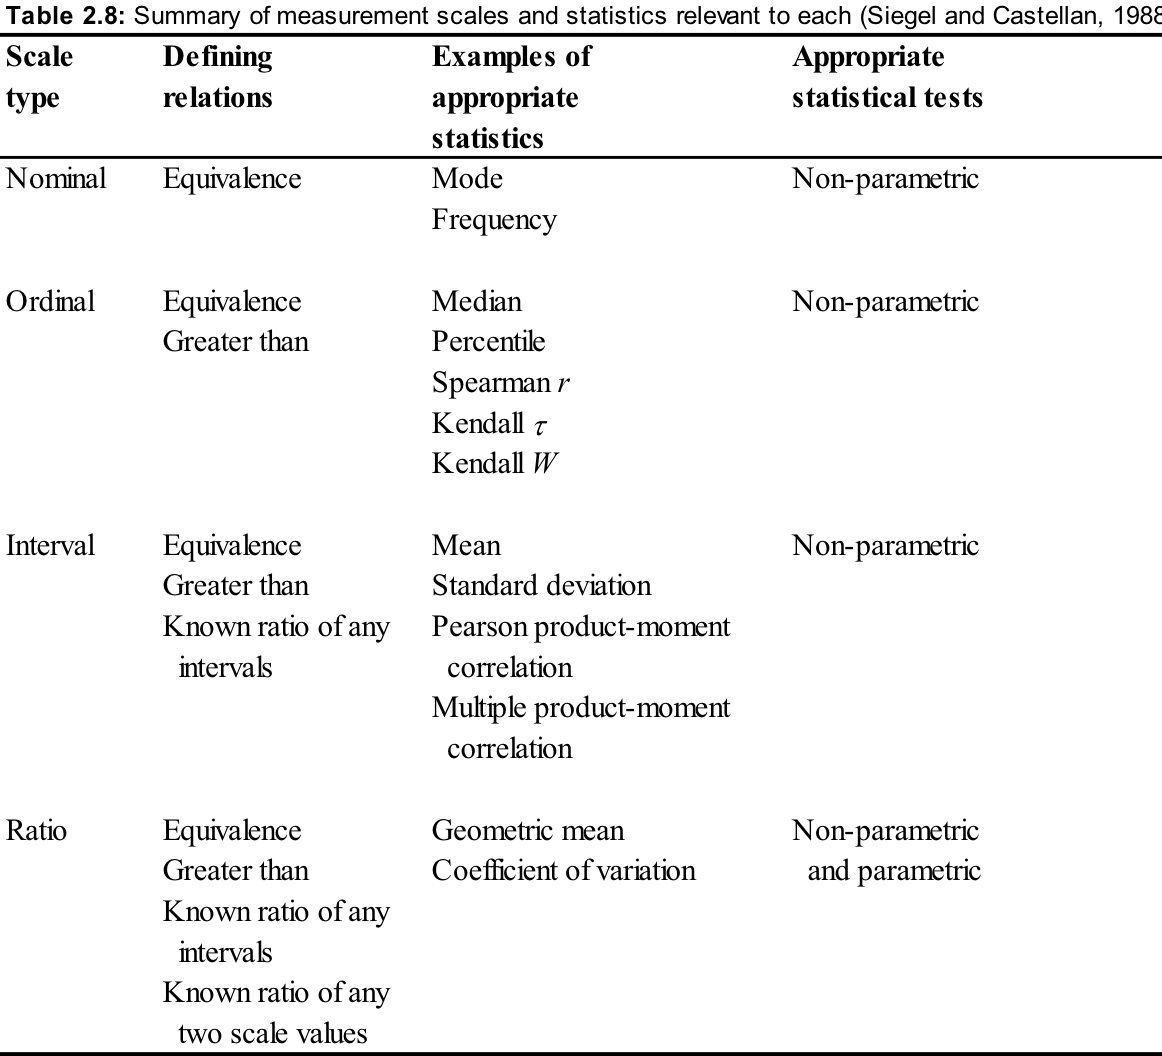
\includegraphics[width=80mm]{A2022.ScaleDeiDati/img-img15.png}
\end{center}

\end{frame}
%=============================================

%---------------------------------------------
\begin{frame}{\centerline{Acceptable Mappings}}

\begin{itemize}
\item For nominal, any 1:1 mapping is OK
\item For ordinal, the mapping needs to be strictly increasing
\item For interval, the mapping must have the form\\ 
\(Y = aX + b\), with \(a > 0\)
\item For ratio, the mapping must have the form\\
\(Y = aX\), with \(a > 0\)
\item For absolute, the only acceptable mapping is\\
\(Y = X\)

\end{itemize}

\end{frame}
%=============================================

%---------------------------------------------
\begin{frame}{\centerline{Examples of Mappings}}

\begin{center}
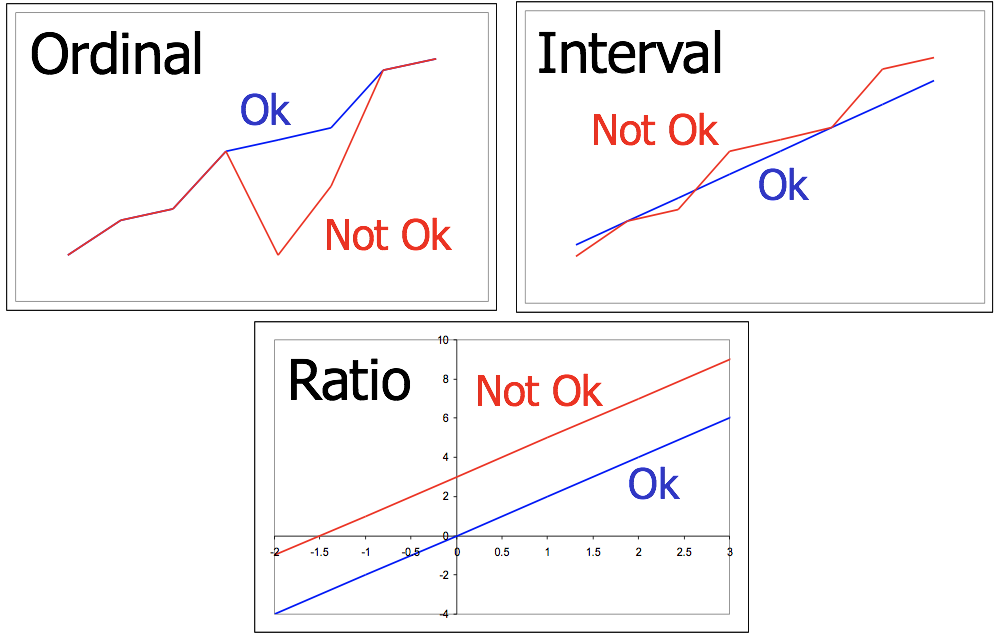
\includegraphics[width=110mm]{A2022.ScaleDeiDati/img-img16.png}
\end{center}

\end{frame}
%=============================================

%---------------------------------------------
\begin{frame}{\centerline{Meaningful Measures}}

\begin{itemize}
\item Measures are said to be meaningful if their truth value does not change when the measure is subject to transformation
\item That is, they are defined on the appropriate scale. Mapping is used to verify the appropriateness of the scale.
\end{itemize}

\end{frame}
%=============================================

%---------------------------------------------
\begin{frame}{\centerline{Examples}}

\begin{table}[H]
\begin{tabulary}{\textwidth}{m{5.5cm} | m{5.5cm}}
\textbf{Meaningful} & 
\textbf{Not meaningful}  \\ \hline

\begin{itemize}    
\item The number of atoms in solid A is double the number of atoms in solid B
\end{itemize} &
\begin{itemize}    
\item The color of solid A is twice as black as the color of solid B
\end{itemize} \\ \hline

\begin{itemize}    
\item The number of people who agreed was double the number of people who disagreed
\end{itemize} &
\begin{itemize}    
\item People agreed twice as much as they disagreed
\end{itemize} \\ \hline

\end{tabulary}
\end{table}

\end{frame}
%=============================================

%---------------------------------------------
\begin{frame}{\centerline{Kinds of metrics}}

\begin{itemize}    
\item A metric is \underline{objective} if it can be taken by an automated device; it is \underline{subjective} otherwise
\begin{itemize}
    \item \textit{LOC are objective metrics, Function Points are subjective}
\end{itemize}
\item A metric is \underline{direct} if it can be directly detected, \underline{indirect} if it is the result of mathematical elaboration on other metrics
\begin{itemize}
    \item \textit{LOC, number of errors, and FP are direct}
    \item \textit{Number of errors per LOC (Error density) is indirect}
\end{itemize}
\end{itemize}
\end{frame}
%=============================================

%---------------------------------------------
\begin{frame}{\centerline{Direct and Indirect Measurement}}

\begin{center}
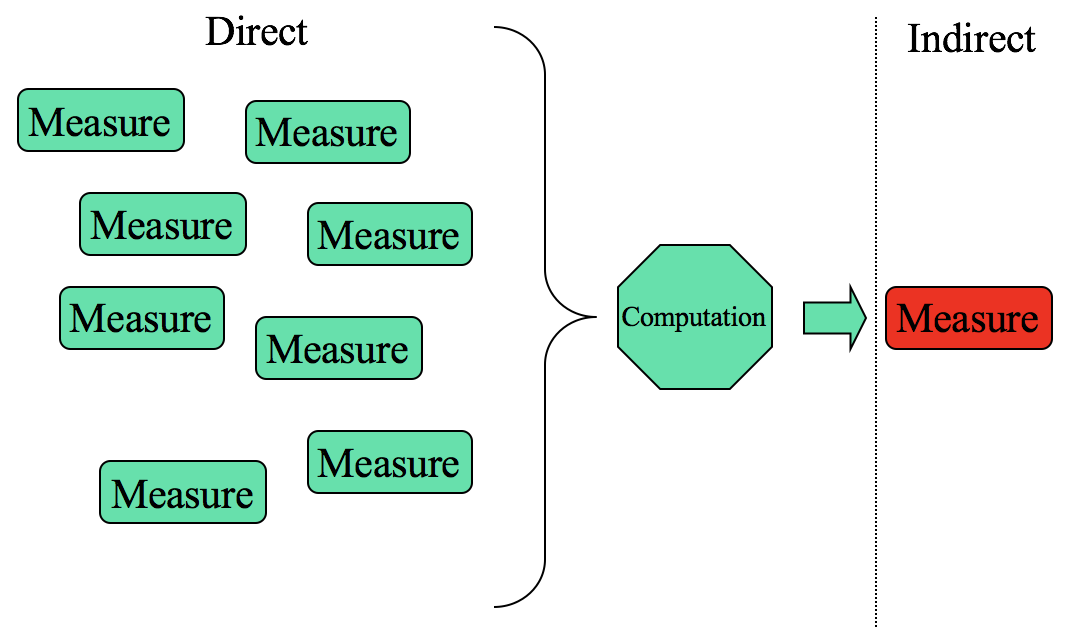
\includegraphics[width=110mm]{A2022.ScaleDeiDati/img-img17.png}
\end{center}

\end{frame}
%=============================================

%---------------------------------------------
\begin{frame}{\centerline{Direct or Indirect}}

\begin{table}[H]
\begin{tabulary}{\textwidth}{m{6cm} m{5cm}}
\begin{itemize}    
\item Immediately definable on one single calculation. Example: LOC, number of people in classroom, number of customer complaints
\end{itemize} &
\begin{itemize}    
\item Derived from a varied set of values. Example: ROI, number of tennis balls by weight, customer satisfaction
\end{itemize}
\end{tabulary}
\end{table}

\end{frame}
%=============================================

%---------------------------------------------
\begin{frame}{\centerline{Measurements, Statistics and Scales}}

\begin{itemize}    
\item Measurement scales limit the type of operations on measure - e.g., central tendency
\item Objective or subjective measurement may limit the type of operations on measures
\item Indirect measure depend on other measures’ scales and thus are limited in meaningfulness and operations
\end{itemize}

\end{frame}
%=============================================

%---------------------------------------------
\begin{frame}{\centerline{Exercise: Measure of Mass}}

\begin{center}

\includegraphics[width=70mm]{A2022.ScaleDeiDati/img-img18.png}
\end{center}
\begin{itemize}    
\item What are the relations between their masses?
\item Which of these are valid mappings?
\begin{itemize} 
    \item \(M_1(A)=1,\)  \(M_1(P)=130,\) \(M_1(E)=1400\)
    \item \(M_2(A)=3,\)  \(M_2(P)=4,\) \(M_2(E)=5\)
    \item \(M_3(A)=24,\) \(M_3(P)=51,\) \(M_3(E)=49\)
\end{itemize}
\item Can we tell how intelligent they are from these mappings?

\end{itemize}
\end{frame}
%=============================================

%---------------------------------------------
\begin{frame}{\centerline{Questions}}

\begin{itemize} 
\item Is it wrong to assert that ``lines of code'' is a bad software measure?
\item What scale is used in ``lines of code'' measurement?
\item Discuss the notion of ``distance'' in a vector space and its meaningfulness as a measure
\item What kind of measure would you use for ``program quality?''
\end{itemize}

\end{frame}
%=============================================

%---------------------------------------------
\begin{frame}{\centerline{Building Models out of Metrics}}

\begin{itemize} 
\item A baby should double its weight at the age of month 6.
\end{itemize}
\begin{center}
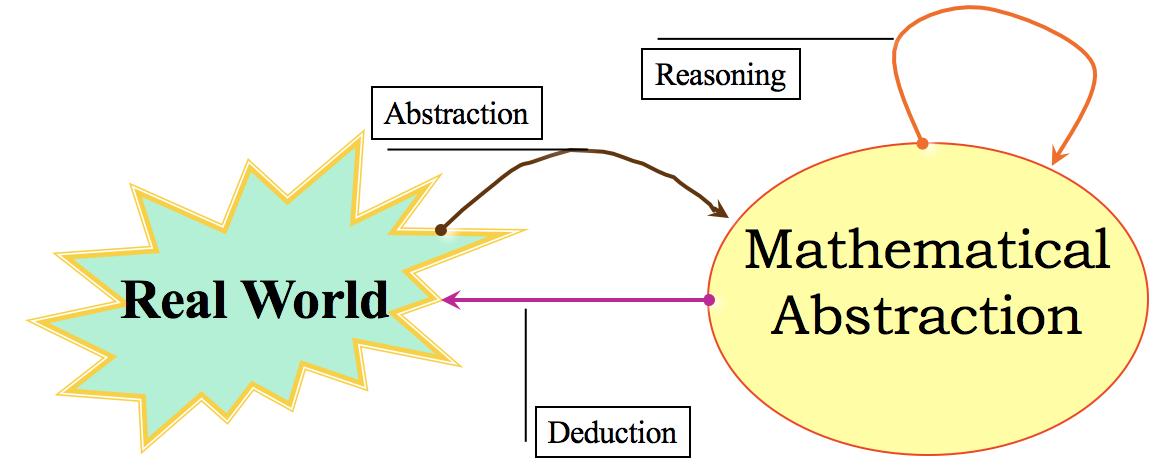
\includegraphics[width=120mm]{A2022.ScaleDeiDati/img-img19.png}
\end{center}
\end{frame}
%=============================================

%---------------------------------------------
\begin{frame}{\centerline{Model}}

\begin{itemize} 
\item Mathematical abstraction
\begin{itemize}
    \item Indirect measurement
    \item Control measurement
    \item Prediction measurement
\end{itemize}    
\item \textbf{Prediction system} couples a model with procedures that allow forecasting
\end{itemize}

\end{frame}
%=============================================

%---------------------------------------------
\begin{frame}{\centerline{Risks while building models}}

\begin{center}
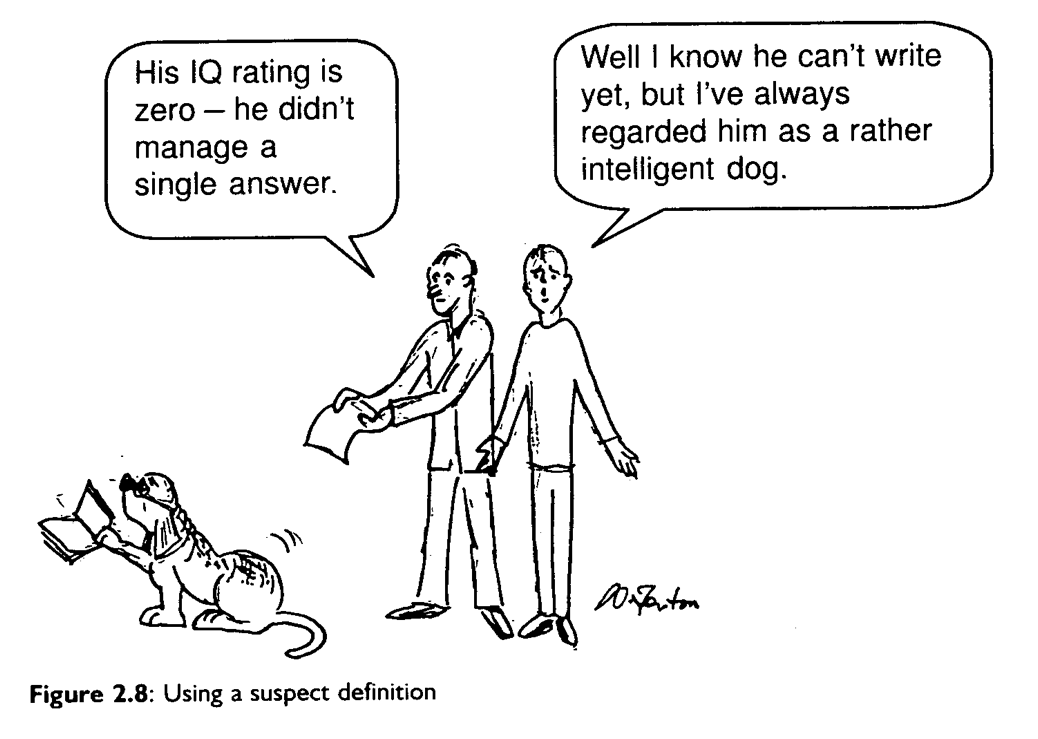
\includegraphics[width=85mm]{A2022.ScaleDeiDati/img-img20.png}
\newline
\end{center}
\begin{small}
\begin{center}
from Fenton pp. 38
\end{center}
\end{small}

\end{frame}
%=============================================

%---------------------------------------------
\begin{frame}{\centerline{Case study}}

\begin{center}
\LARGE
Metrics to assess personal productivity
\end{center}

\vspace{3cm}

{\tiny From:
\url{https://www.analyticsinhr.com/blog/employee-performance-metrics/}
}

\end{frame}
%=============================================

%---------------------------------------------
\begin{frame}{\centerline{The work}}


\begin{itemize}
\item We now analyse how people are evaluating quantitatively the personal productivity. \\
\item The full document is available at the website above. \\
\item We can review it using our approach to metrics. \\
\item We adopt a simplified GQM. \\
\end{itemize}
\end{frame}
%=============================================
%---------------------------------------------
\begin{frame}{\centerline{Goal}}

\begin{center}
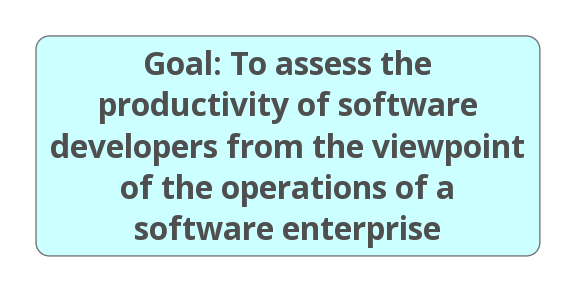
\includegraphics[width=80mm]{A2022.ScaleDeiDati/20180904_CaseStudy_Goal.png}
\newline
\end{center}
{\tiny The text of this and the following slides comes from:
\url{https://www.analyticsinhr.com/blog/employee-performance-metrics/}
}

\end{frame}

%---------------------------------------------
\begin{frame}{\centerline{Questions}}

\begin{center}
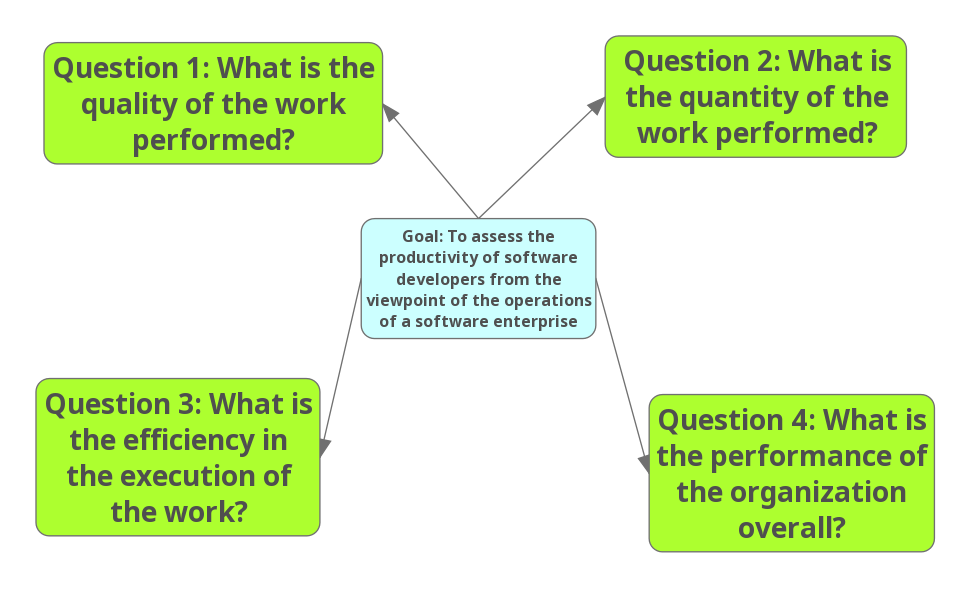
\includegraphics[width=120mm]{A2022.ScaleDeiDati/20180904_CaseStudy_GoalQuestions.png}
\newline
\end{center}

\end{frame}



\begin{frame}{\centerline{Proposed exercise}}


\begin{itemize}
\item Create a mix team of 3 people of which at least one of each gender
\item Complete the GQM with the  metrics
\item For every metrics determine:
\begin{itemize}
\item if it direct or indirect
\item if it is subjective or objective
\item its measurement scale
\end{itemize}
\item Provide a significant subset of the model that you would use to evaluate yourself
\item Write the results on a table distributed on a set of slides in overleaf and send the result to the Telegram group
\begin{itemize}
\item Organize every line as follows:
\begin{itemize}
\item Referred Goal and Question as number, e.g., G1Q2
\item Metrics,
\item Direct or indirect, 
\item Subjective or objective, 
\item Measurement scale
\end{itemize}
\end{itemize}
\end{itemize}
\end{frame}

%---------------------------------------------
\begin{frame}{\centerline{Q1 Metrics (1)}}

\begin{center}
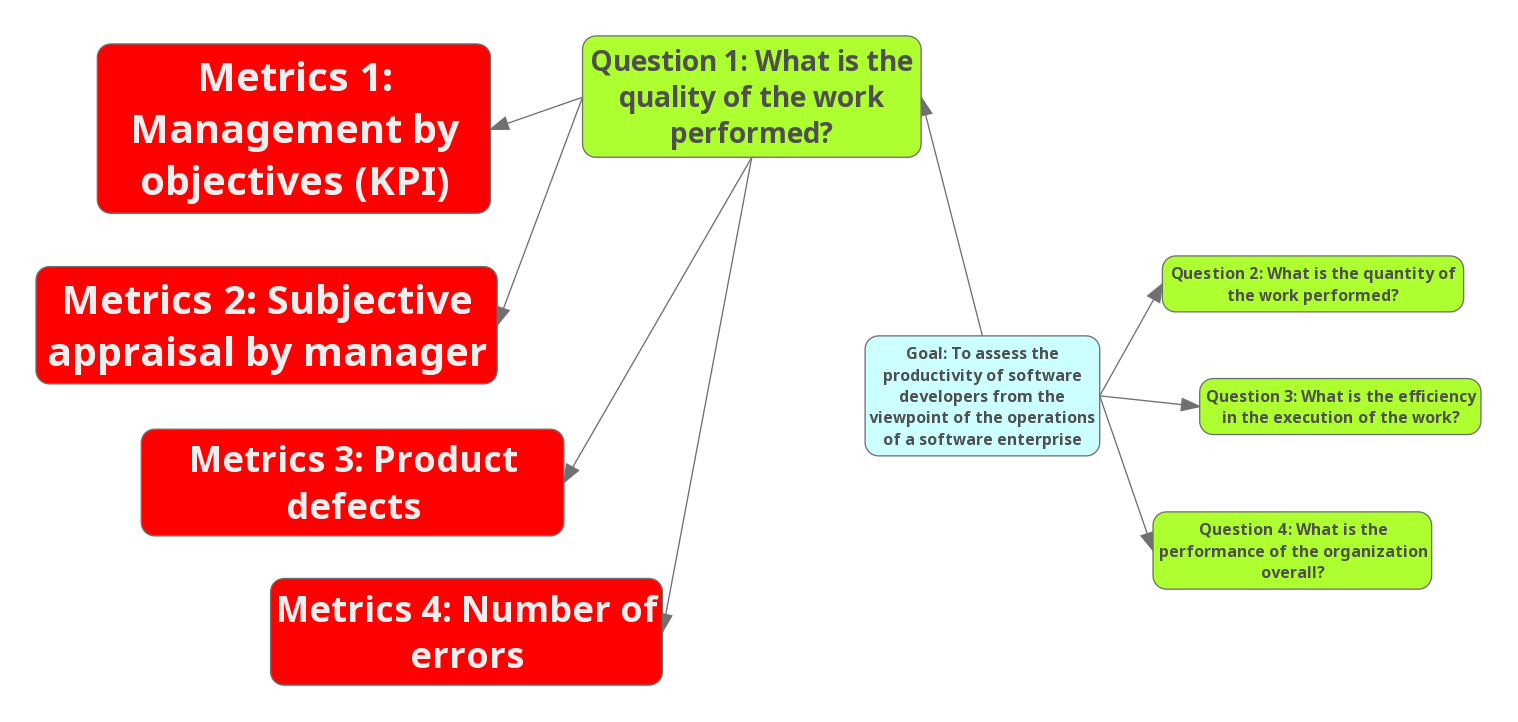
\includegraphics[width=120mm]{A2022.ScaleDeiDati/20180904_CaseStudy_GoalQuestions_M1.png}
\newline
\end{center}

\end{frame}

%---------------------------------------------
\begin{frame}{\centerline{Focus on Q1 M2}}

\begin{center}
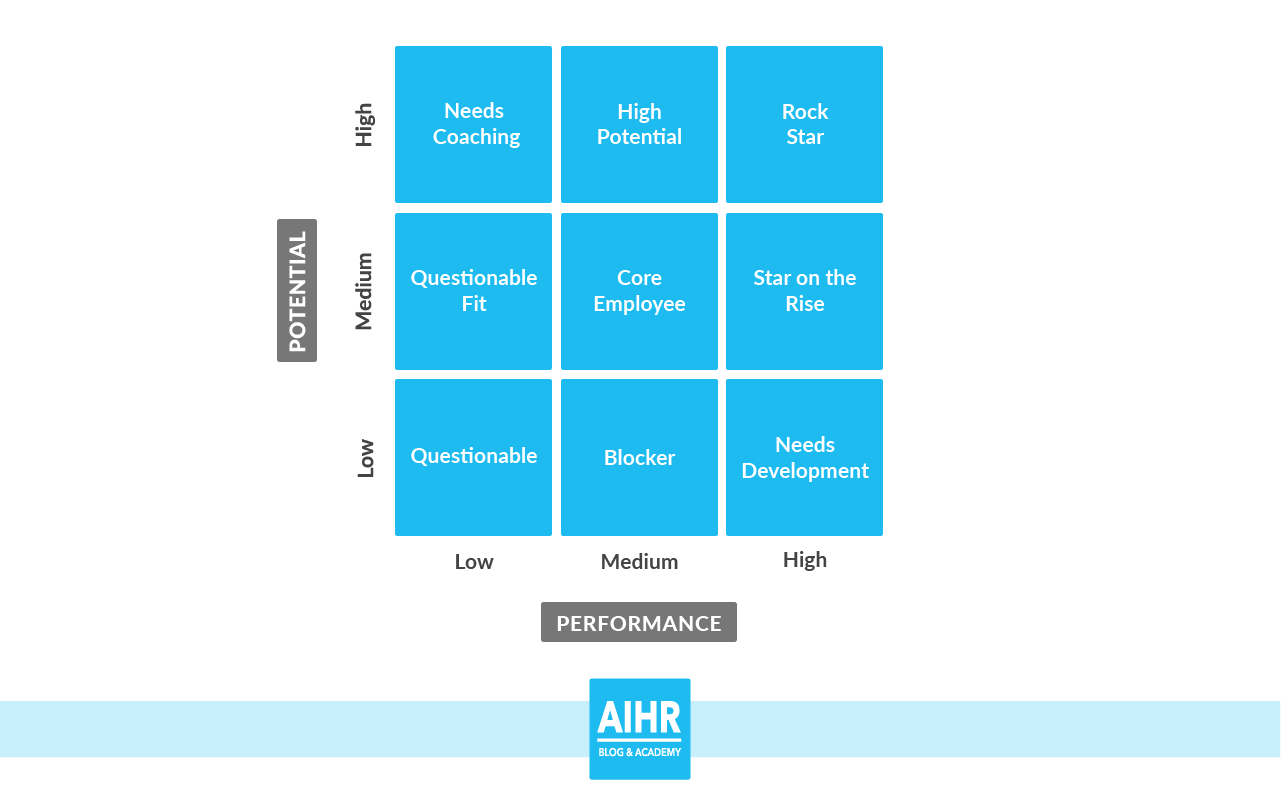
\includegraphics[width=120mm]{A2022.ScaleDeiDati/20180904_CaseStudy_GoalQuestions_M1_SubjectiveApprisalByManager.png}
\newline
\end{center}

\end{frame}

%---------------------------------------------
\begin{frame}{\centerline{Q1 Metrics (2)}}

\begin{center}
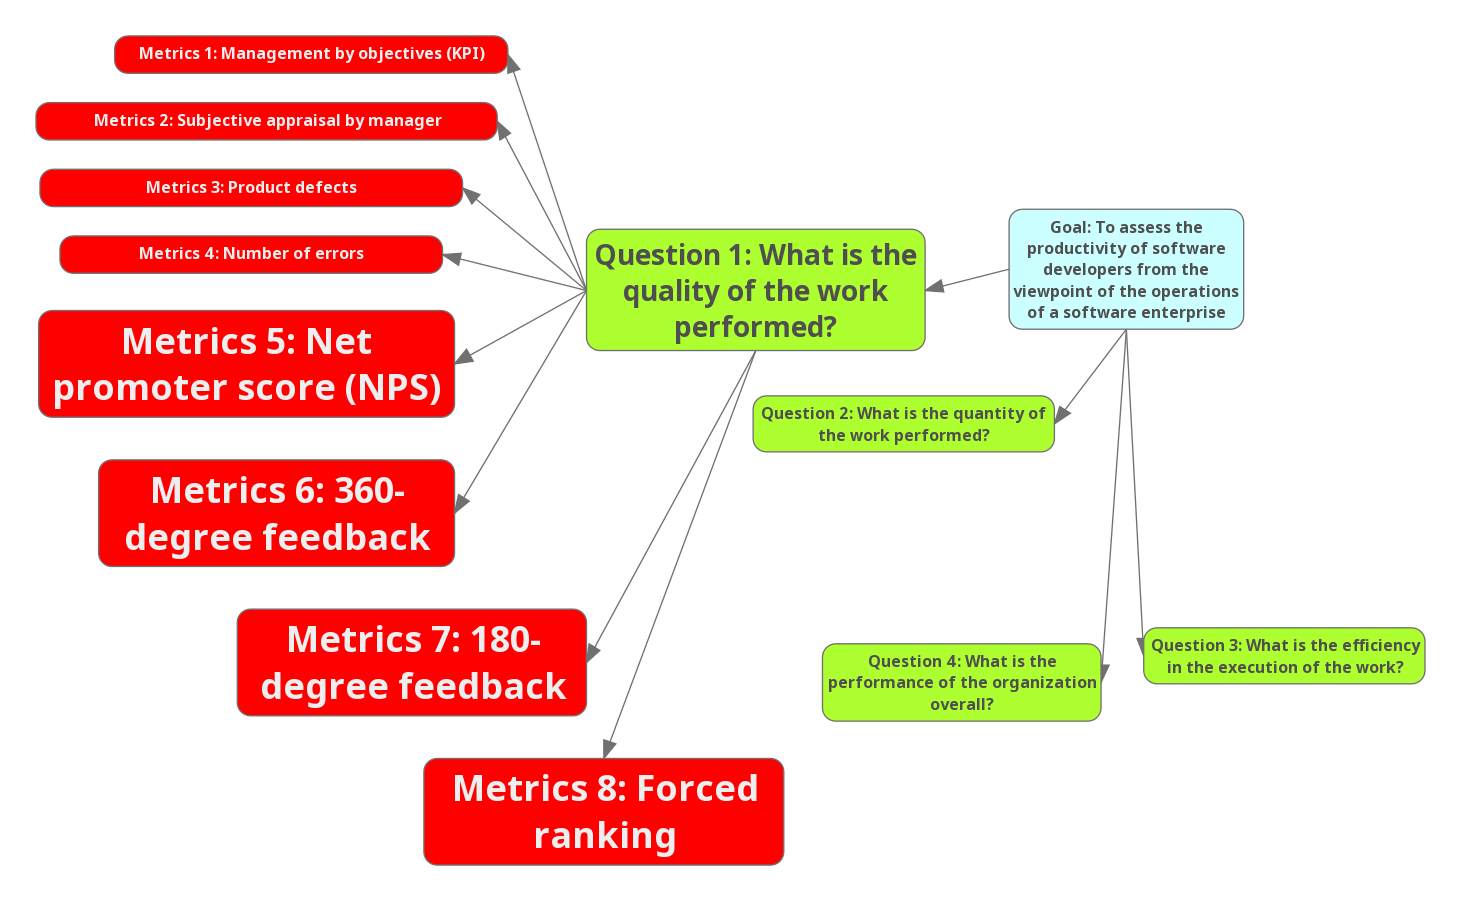
\includegraphics[width=120mm]{A2022.ScaleDeiDati/20180904_CaseStudy_GoalQuestions_M2.png}
\newline
\end{center}

\end{frame}

%---------------------------------------------
\begin{frame}{\centerline{Focus on Q1 M6}}

\begin{center}
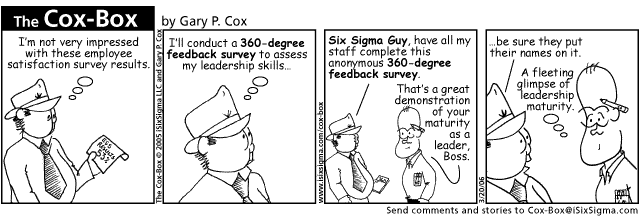
\includegraphics[width=120mm]{A2022.ScaleDeiDati/20180904_CaseStudy_GoalQuestions_M2_360DegreeEmployeePerformanceMetrics.png}
\newline
\end{center}

\end{frame}

%---------------------------------------------
\begin{frame}{\centerline{Q2 Metrics}}

\begin{center}
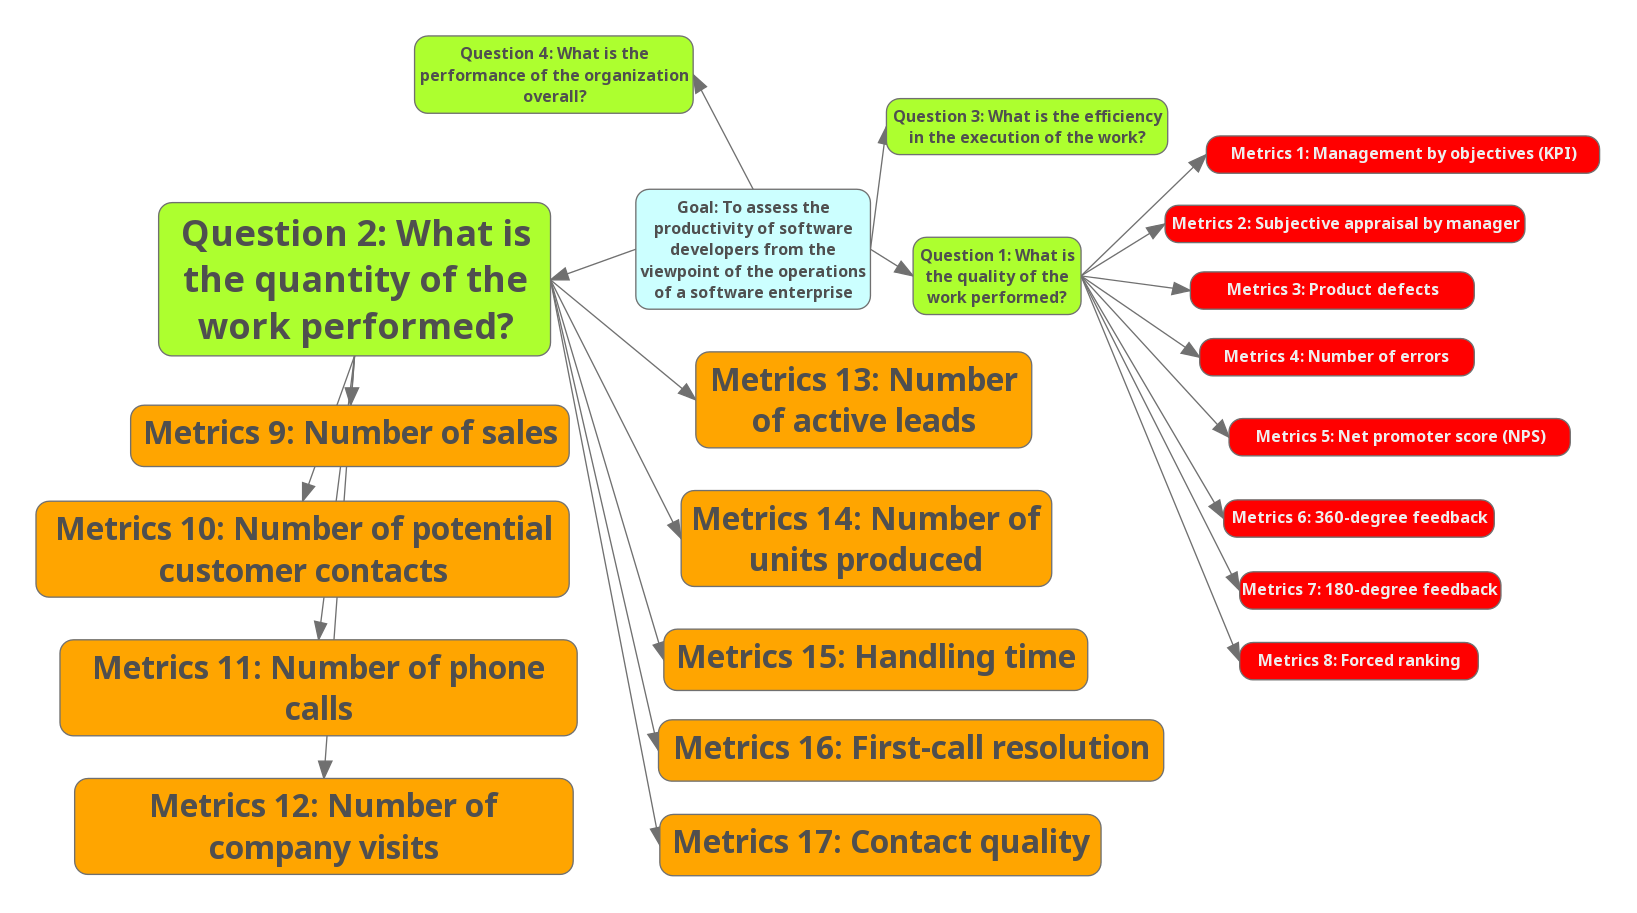
\includegraphics[width=125mm]{A2022.ScaleDeiDati/20180904_CaseStudy_GoalQuestions_M3.png}
\newline
\end{center}

\end{frame}

%---------------------------------------------
\begin{frame}{\centerline{Q3 Metrics}}

\begin{center}
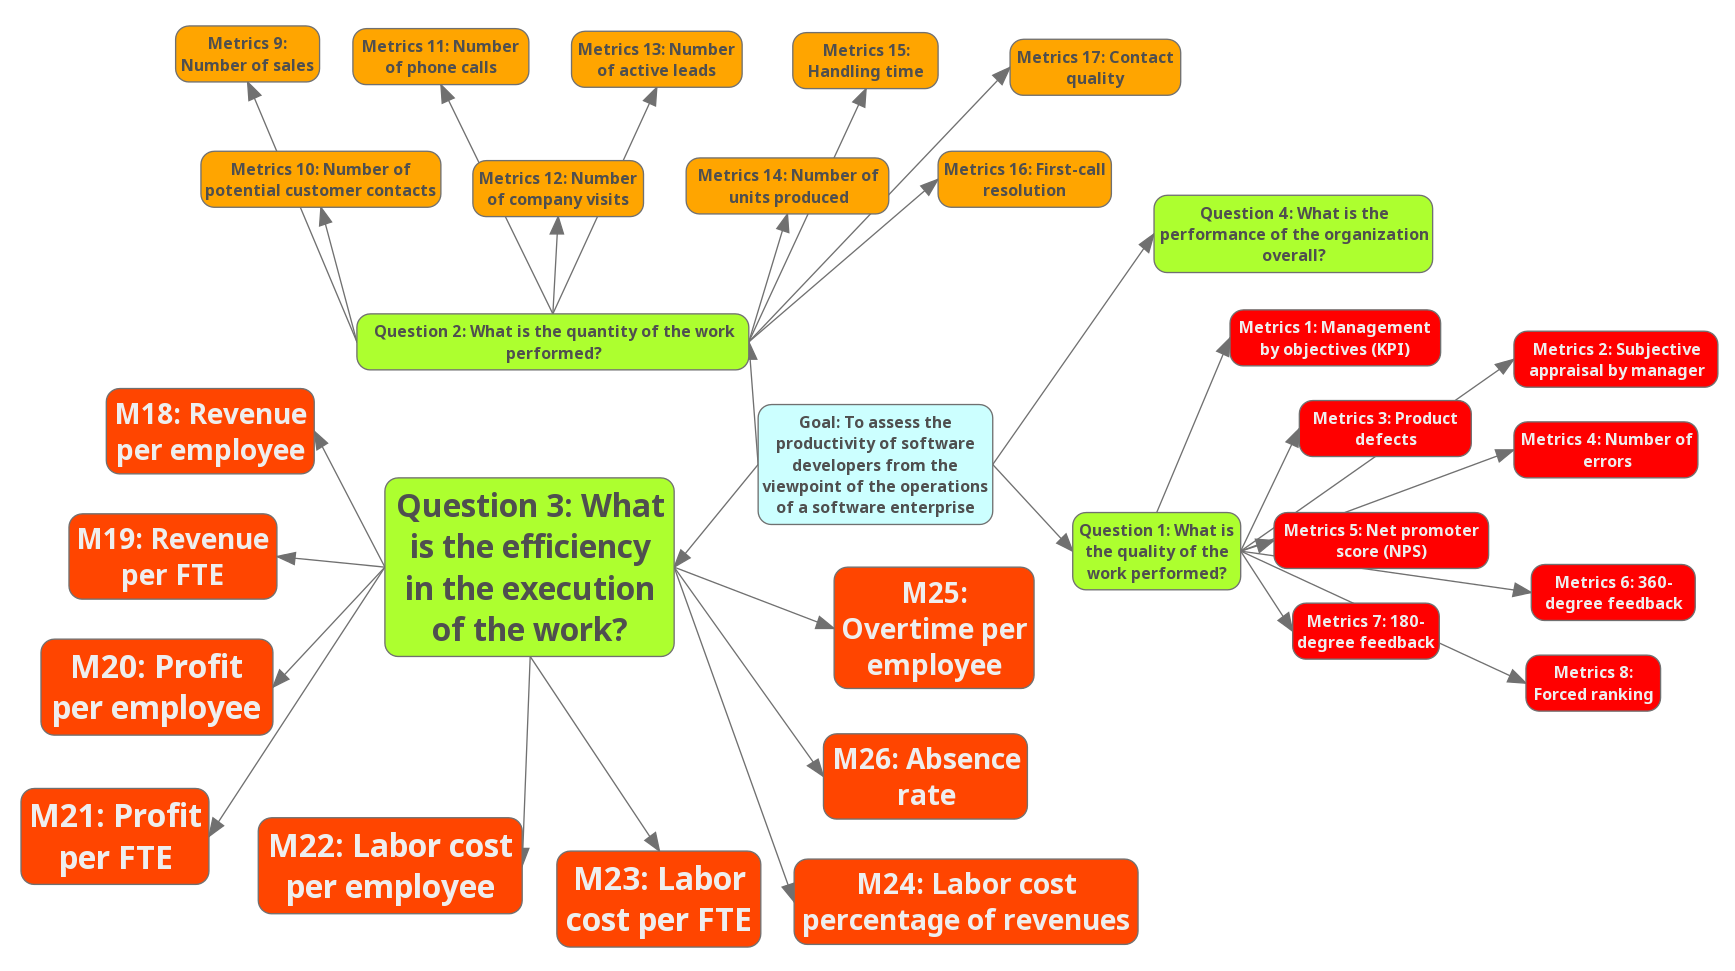
\includegraphics[width=125mm]{A2022.ScaleDeiDati/20180904_CaseStudy_GoalQuestions_M4.png}
\newline
\end{center}

\end{frame}

\begin{frame}
{\centerline{Domande?}}
\vspace{1cm}
\begin{center}
    \LARGE{Fine della lezione sette.}
\end{center}

\end{frame}

\end{document}
